\chapter{Architettura dei DBMS}

Una transazione è un'\textbf{unità di programma}: 
    \begin{itemize}
        \item{Una transazione ha un \textbf{begin transaction} che comunica al DBMS la richiesta di interazione con esso da parte dell'applicazione.}
        \item{Il DBMS identifica l'inizio della transazione $T_i$ e la abbina in modo univoco con l'utente/applicazione che ne ha fatto richiesta.}
        \item{Il DBMS, nell'ambito di $T_i$, riceve dei comandi DML in sequenza e le abbina alla transazione.}
    \end{itemize}

I DBMS gestiscono le transazioni garantendo, per ogni transazione $T_i$, il soddisfacimento delle proprietà $ACID$:
    \begin{itemize}
        \item{Atomicità}
        \item{Consistenza}
        \item{Isolamento}
        \item{Durabilità}
    \end{itemize}

La seguente figura rappresenta un modello di architettura del DBMS:
    \begin{figure}[h!]
        \centering
        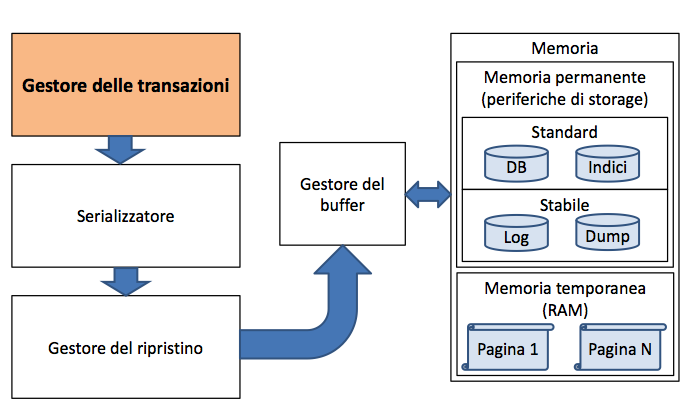
\includegraphics[scale = 0.45]{05/img01}
        \caption{Architettura dei DBMS}
    \end{figure}
    
    
Il \textbf{gestore delle transazioni} riceve le transazioni e ne gestisce il ciclo di vita inviando i comandi DML alle componenti sottostanti che devono eseguire l'azione richiesta.\\\\
Il \textbf{serializzatore} è responsabile della proprietà di \textit{isolamento} (quando il programmatore progetta una transazione, lo fa nell'ipotesi che il DBMS la esegua in modo isolato rispetto alle altre transazioni).\\\\
Il \textbf{gestore del ripristino}, oltre a gestire il ripristino in seguito a guasti, è responsabile della proprietà di \textit{atomicità} (la transazione dev'essere eseguita interamente o per nulla).\\
Il gestore del ripristino garantisce anche l'\textit{integrità} dei dati (se i dati vengono corrotti, il gestore del ripristino cerca di recuperare il dato corretto oppure forza un abort della transazione).\\\\
Il \textbf{gestore del buffer} è responsabile della \textbf{durabilità} (persistenza dei dati del DBMS).\\\\
La \textbf{consistenza} è di competenza sia del \textbf{gestore delle transazioni} (verifica di tutti i vincoli della base di dati) che del serializzatore.

\section{Memoria centrale}
Consideriamo la nostra area di lavoro, cioè la memoria centrale.\\
Nell'area di lavoro abbiamo la transizione $T_i$ che richiede la lettura/modifica di un record. Quando una transizione richiede l'attività su un record, invia delle richieste al gestore del buffer.\\
La transazione $T_i$ invia una richiesta chiamata \textbf{fix pid}, che significa: la transazione ha bisogno di avere a disposizione una pagina dati di indirizzo \textbf{pid}.

\subsection{Le pagine}
Tutti i dati del database (tabelle, indici, log e dump) sono organizzati in pagine.\\
Le pagine hanno dimensioni che dipendono dal sistema (anche variabili), e contengono i record.\\
Se la transazione ha bisogno di lavorare su un ben determinato record (tupla), bisogna cercare una pagina con un certo indirizzo \textbf{pid} che si presume contenga il record desiderato.

\subsubsection{Caricamento delle pagine}
La transazione per lavorare su un dato ha sempre bisogno di chiedere al buffer la disponibilità di una precisa pagina:
    \begin{enumerate}
        \item{Il \textbf{gestore del buffer} caricherà la pagina nel buffer stesso, prendendola dalla periferica di storage se non già presente nel buffer.}
        \item{Il gestore del buffer prende i dati memorizzati nel disco (settori di tracce sul disco) e li mette nella cache presente nella periferica stessa.}
        \item{Dalla cache vengono poste nel buffer della memoria centrale.}
        \item{Il gestore del buffer risponde alla transazione inviandole l'indirizzo della memoria centrale in cui trovare la pagina.}
        \item{La transazione acquisisce, tramite il comando \textbf{fix pid}, il puntatore alla zona di memoria (buffer) che contiene la pagina.}
        \item{In caso di lettura, si accontenta di leggere i dati.}
        \item{In caso di scrittura o modifica, avviene il processo inverso, ovvero, la transazione modifica i dati \textit{nel buffer}.}
        \item{È il gestore del buffer che si occupa di copiare la pagina con le modifiche nella periferica.}
    \end{enumerate}

\subsubsection{Semplificazione}
La pagina è composta da un certo numero di blocchi fisici, che a loro volta sono composti da un certo numero di settori.\\
In questo corso, però, confonderemo il blocco fisico con la pagina (dimensione blocco = dimensione pagina).\\\\
Le dimensioni caratteristiche dei blocchi fisici vanno dai 512 Byte ai 4KB, mentre le dimensioni delle pagine vanno dai 4KB agli 8KB.\\
Il dimensionamento della pagina è importante perché influisce sulle prestazioni dell'intero DBMS.

\subsubsection{Tempi di trasferimento}
Ricordiamo che i tempi di trasferimento di una pagina tra periferiche di storage e RAM (e viceversa) sono dell'ordine dei millisecondi ($10^{-3} s$).\\
I tempi di trasferimento di pagine in RAM sono dell'ordine dei nanosecondi ($10^{-9}$ s).\\\\
Il fattore di differenza è $10^6$: dunque, il costo temporale è tutto sulla movimentazione delle pagine dalla periferica alla memoria centrale (e viceversa).\\\\
Nonostante i progressi tecnologici, il divario ha ancora lo stesso ordine di grandezza.

\subsubsection{Struttura di una pagina}
La pagina contiene:
    \begin{itemize}
        \item{\textbf{Array degli offset}}
        \item{\textbf{Contatore CP}: conta i programmi che hanno avuto l'OK di accesso alla pagina}
        \item{\textbf{Set Dirty Bit}: vale 1 se la pagina è stata modificata.}
        \item{\textbf{Stack dei records}: ontenuto della pagina.}
        \item{\textbf{Bit di parità}}
    \end{itemize}
Per l'identificazione di un record è necessario fornire due valori:
    $$RID[PID, i]$$
Dove $PID$ è l'identificatore della pagina, mentre $i$ è un offset.\\
L'architettura di $RID$, con indice e offset, consente al gestore delle pagine (il filesystem) di modificare la posizione dei records a piacimento all'interno dell'area dati senza influenzare gli indirizzi esterni.